\documentclass[a4paper,11pt,twocolumn]{paper}
\usepackage{fullpage}
\usepackage[latin1]{inputenc}
\usepackage[T1]{fontenc}
\usepackage[normalem]{ulem}
\usepackage[english]{babel}
\usepackage{listings,babel}
\lstset{breaklines=true,basicstyle=\ttfamily}
\usepackage{graphicx}
\usepackage{moreverb}
\usepackage{float}
\usepackage{cite}
\usepackage{nopageno}

\title{Technical overview of Milkymist SoC}
\subtitle{Revision F (Apr. 2011)}
\author{S\'ebastien Bourdeauducq}
\begin{document}
\maketitle{}
\section{Introduction}
The Milkymist\textsuperscript{\texttrademark} project~\cite{milkymist} develops a stand-alone device in a small form factor that is capable of rendering MilkDrop-esque visuals effects~\cite{milkdrop} in real time, with a high level of interaction with many sensors and using live audio and video streams as a base.

The flexibility of the FPGA used as a central component enables advanced users to modify the design, and also permits compact integration of many interfaces (Ethernet, USB, MIDI, DMX512, IR remote, video input), making Milkymist\textsuperscript{\texttrademark} a platform of choice for the mobile VJ.

But Milkymist\textsuperscript{\texttrademark} is more than a visual synthesizer - it is also developing and maintaining one of the leading open source system-on-chip designs. It is today the fastest open source system-on-chip capable of running uClinux, and it comes with an extensive set of features and graphics accelerators.

The IP cores that make up the system-on-chip are entirely written in open source synthesizable Verilog HDL with extensive use of logic inference to ease porting to various FPGA and ASIC technologies. They come with test benches and documentation. This makes Milkymist\textsuperscript{\texttrademark} a great library of re-usable logic cores to serve as a base for other open source hardware.

\begin{figure}
\centering
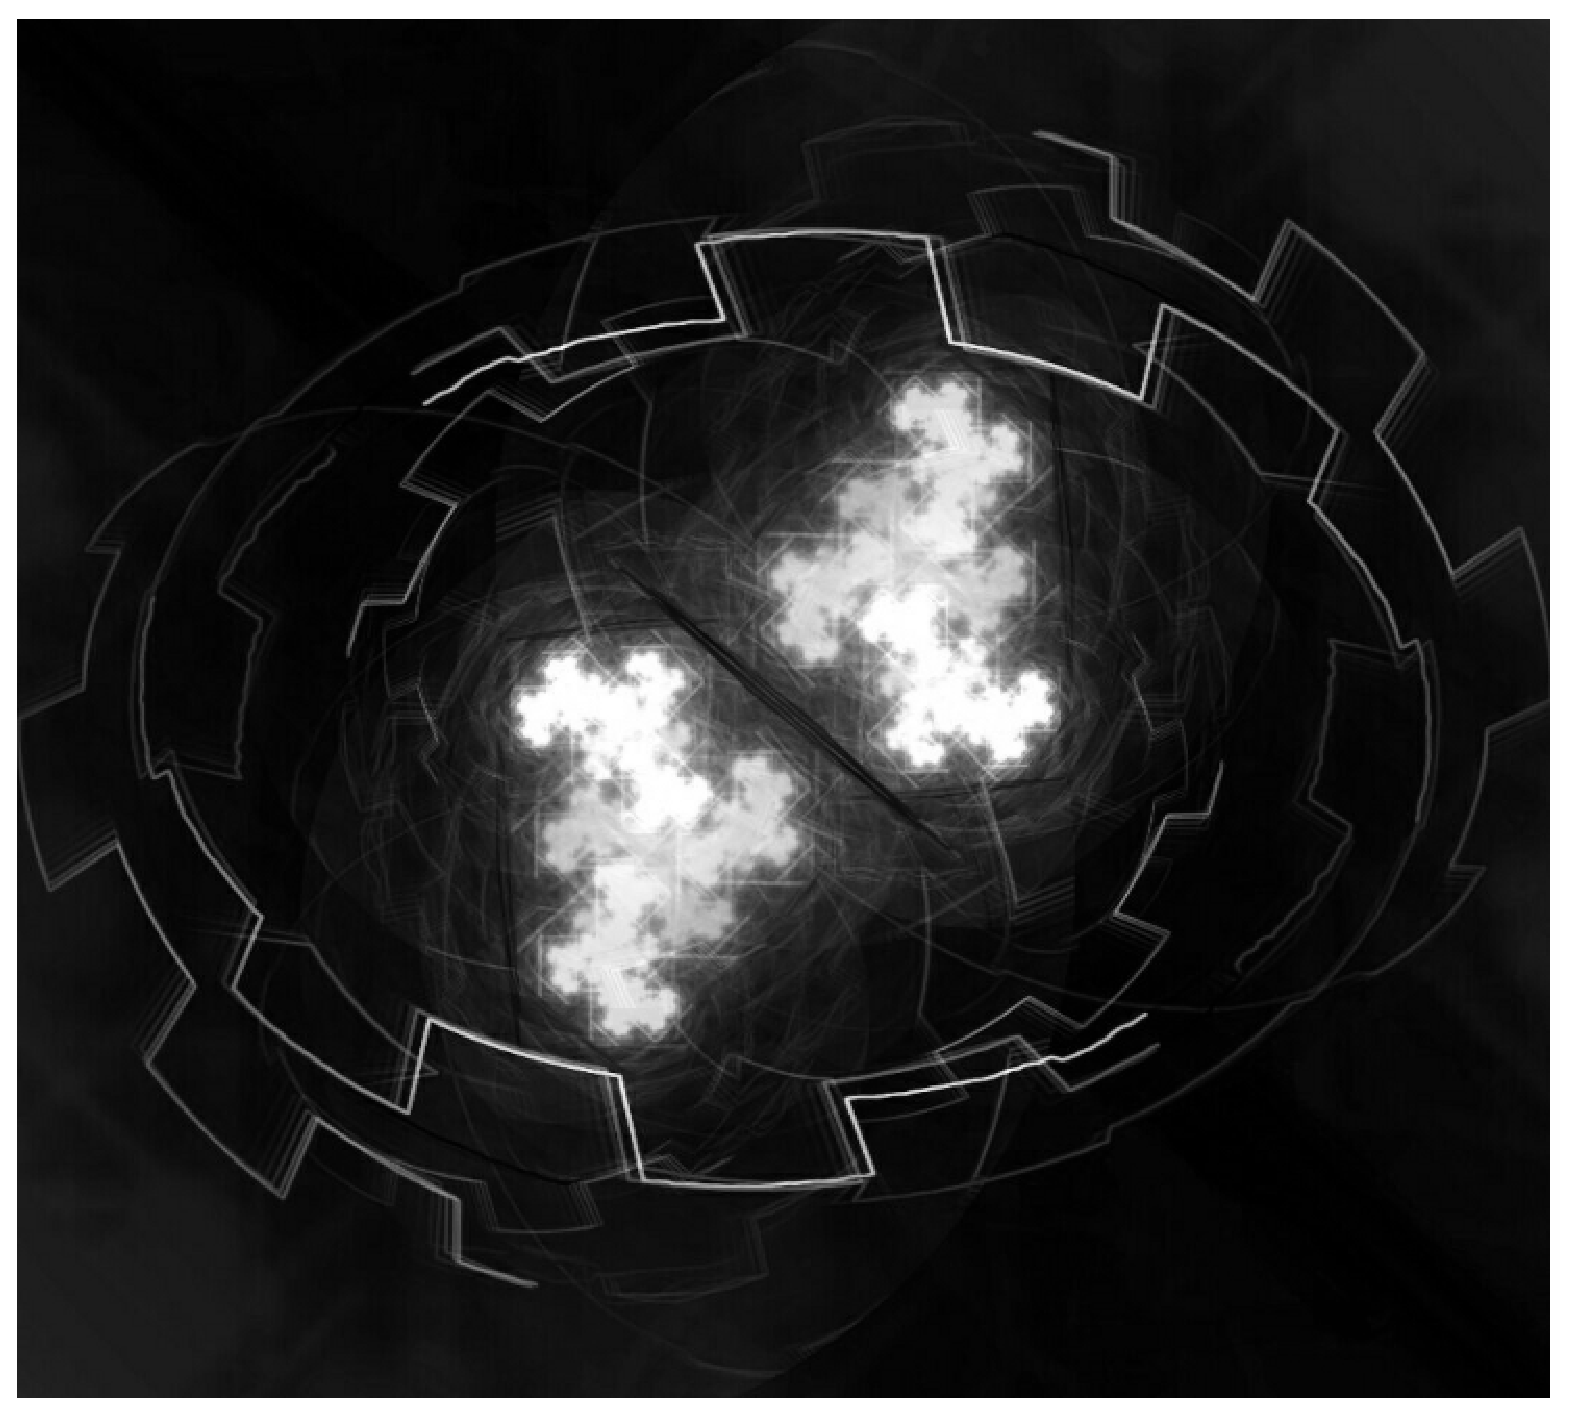
\includegraphics[height=60mm]{milkdrop_bw.eps}
\caption{Sample video output from MilkDrop}
\label{fig:genodefx}
\end{figure}

This paper gives a technical overview of the system-on-chip and its environment.

\section{System architecture}
The block diagram of the complete system-on-chip is given in Figure~\ref{fig:block}. The complete system is written in synthesizable Verilog HDL. Its components are detailed below.
\begin{figure*}
\centering
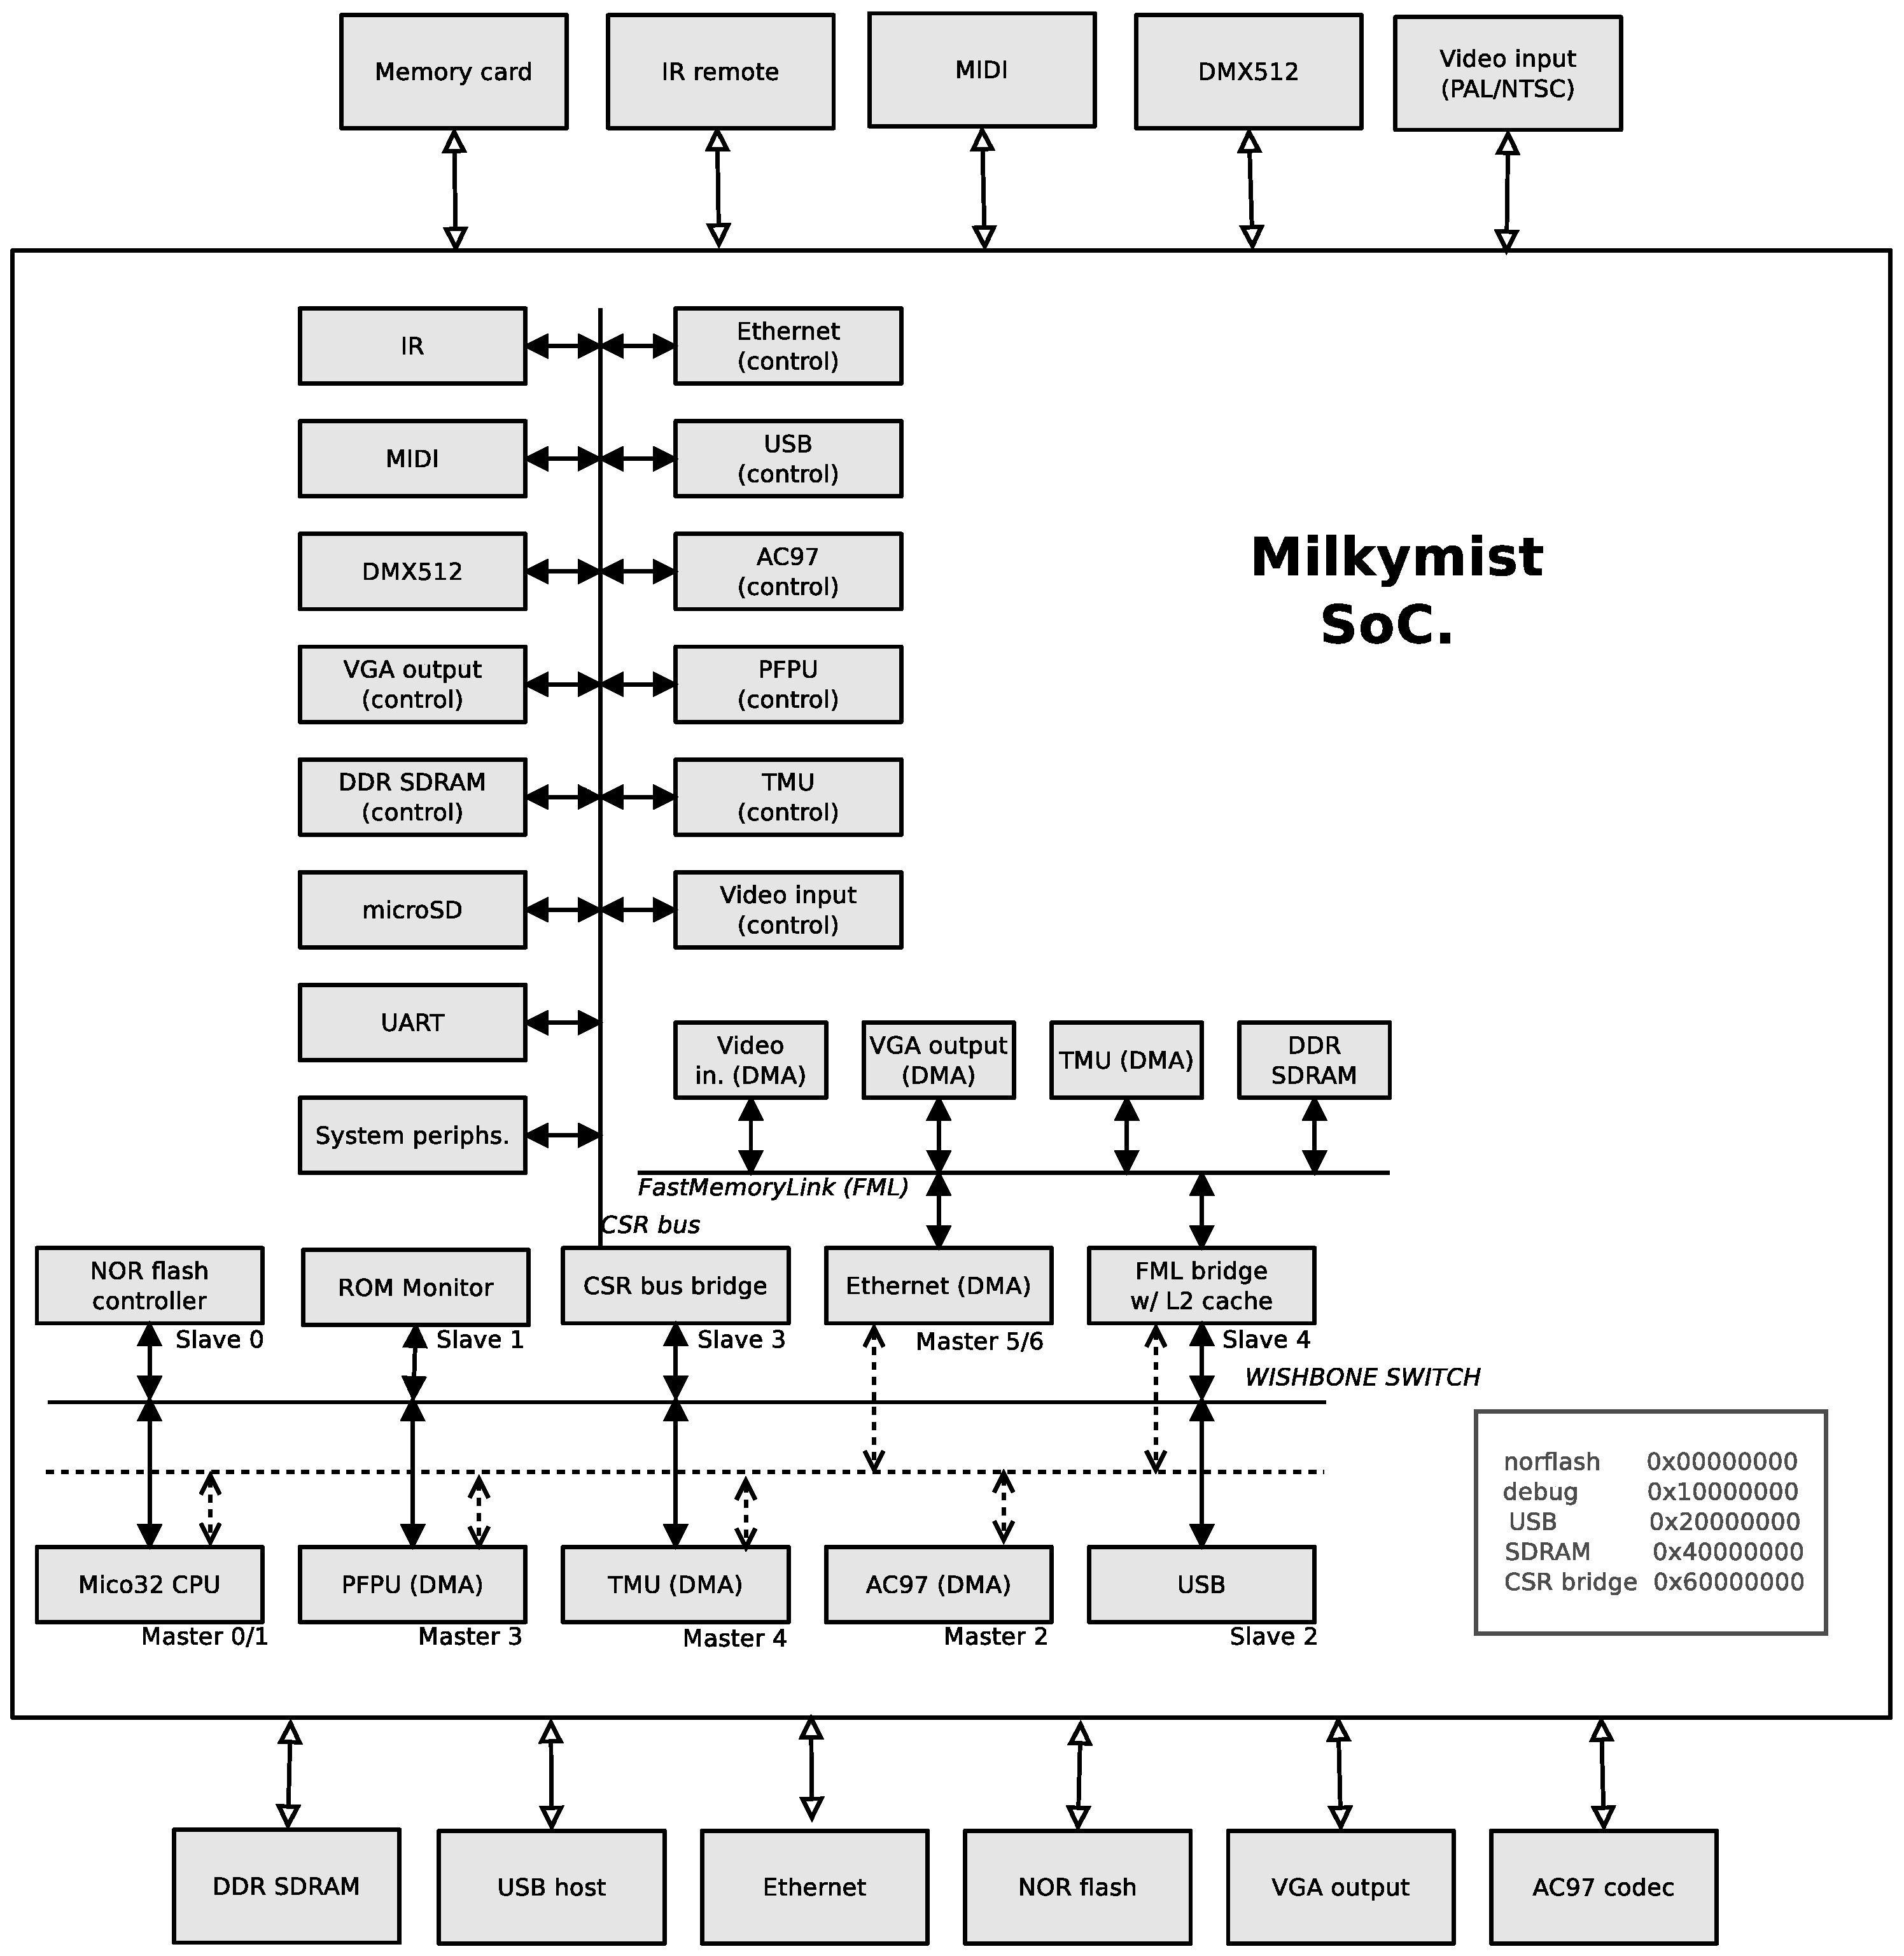
\includegraphics[width=\textwidth]{soc_architecture.eps}
\caption{SoC block diagram}
\label{fig:block}
\end{figure*}

\subsection{SoC interconnect}
The Milkymist system-on-chip uses three different kind of buses :
\begin{itemize}
\item WISHBONE~\cite{wishbone} as a general purpose bus around the CPU core.
\item a custom ``CSR'' bus~\cite{csr} used to access configuration and status registers of peripherals. It is simpler than WISHBONE; it does not support variable latency and the address decoding is simplified.
\item a custom ``FastMemoryLink'' (FML) bus~\cite{fml} which is pipelined and burst-oriented for efficient DRAM access.
\end{itemize}
By removing the need for logic that is only required to comply with a too general bus specification, the use of these specific buses reduce the hardware design effort and improve resource efficiency.

\subsection{Building blocks}
\subsubsection{Base system}
The base system is made up of a LatticeMico32 CPU core~\cite{mico32}, on-chip SRAM, off-chip Flash, an UART for printing debug messages, general-purpose I/O ports, timers, and interrupt controller.

The LatticeMico32 core can execute uClinux~\cite{micolinux}, or be programmed like a microcontroller, without operating system. Early versions of the system-on-chip used AEMB~\cite{aemb} instead of LatticeMico32. It has been replaced because of performance and software support complexity reasons.

These make up a basic system that is capable of executing software and communicate with the outside world. On top of this system, special peripherals and accelerators are added.

\subsubsection{Memory interface}
The system-on-chip is equipped with a custom DDR SDRAM controller~\cite{hpdmc}, supporting a FastMemoryLink interface.

The DDR SDRAM data bus width is 32 bits and is running at up to 100MHz, delivering a peak (ideal) memory bandwidth of 6.4Gbps.

The memory controller is fully synchronous (the SDRAM clock is the system clock) to avoid clock domain crossing delays and reduce the overall memory latency.

It is a ``page mode'' controller, which leaves DRAM pages open after an access on the chance that the next access will be on the same page. This has been shown to be fruitful in most cases~\cite{pagemode}.

Memory latencies are further reduced by the use of pipelined transfers on the FML bus.

\subsubsection{VGA output}
The system-on-chip directly drives the H/V synchronization pins of the VGA interface and a video DAC that generates the red, green and blue analog signals.

The framebuffer is read from DRAM using the FML interface directly.

To cope with the hard realtime constraint of the video signal generation, the VGA controller contains a FIFO which hides the memory latencies.

The framebuffer uses a simple progressive scan 16bpp RGB565 schema. The controller supports multiple buffering and synchronizes the switching between the framebuffers with the vertical blanking intervals in order to prevent drawing artifacts.

\subsubsection{Texture mapping unit (TMU)}
The unit maps a texture on a rectangular surface with texture coordinates defined on a grid of control points. It supports bilinear filtering, texture wrapping, alpha blending, additive drawing, and chroma keying.

To implement MilkDrop at a good frame rate, this becomes a very computation and memory intensive process. The implementation is heavily parallel, and is directly connected to the FML bus to acheive memory bandwidth constraints~\cite{confslides}~\cite{tmu}.

\subsubsection{Programmable floating point unit (PFPU)}
The PFPU~\cite{pfpu} is a floating point coprocessor, whose primary purpose is generating vertex data when implementing MilkDrop. It is similar to the vertex shader of traditional graphics processing units.

It is a pipelined VLIW processor with all the scheduling done by the compiler. This radical approach enables a very efficient use of the FPGA resources. Loop structures are not programmable, which limits the use case to evaluating mathematical expressions.

\subsubsection{Audio I/O}
The audio controller interfaces the system-on-chip to industry-standard and cheap AC97 codecs.

It supports full-duplex audio operation at a 16-bit 48kHz sample rate and access to the AC97 codec registers.

\subsubsection{Memory card}
The system is equipped with a memory card controller compatible with the popular memory cards, which are used to store firmware, user media and data.

\subsubsection{Ethernet}
The Milkymist SoC can connect to industry-standard Ethernet PHYs to enable TCP/IP network connectivity and specifically the OpenSoundControl protocol which supersedes MIDI for the connection of electronic instruments.

\subsubsection{USB}
The system-on-chip integrates a protocol stack compatible with full-speed host USB. The SoC connects directly to USB transceivers to interface the ports.

The USB-compatible ports allow connection of keyboards, mice, USB sticks, wireless network cards, etc.

\subsubsection{DMX512 and MIDI}
These two interfaces are common in stage environments. DMX512 is a protocol for controlling lighting while MIDI connects electronic instruments together.

By integrating these two interfaces, the Milkymist SoC enables new ways of easily interacting with the visuals.

\subsubsection{IR remote}
The SoC integrates a RC-5 compatible IR remote control decoder. The user can utilize most electronic appliances' remote controls to interact with the visuals or navigate through GUI menus.

\subsubsection{Video input}
A video input compatible with PAL, SECAM and NTSC is supported by the system. Like every high-bandwidth DMA master, it is connected to the FML bus.

An external ADC and decoder chip with a BT.656 interface like the ADV7181 is used. This simplifies greatly the problem of decoding multiple video standards.

This video input enables the use of the device in live video mixing and transformation applications.

\section{Hardware development system}
The Milkymist SoC is the central component of our commercial Milkymist One product (figures~\ref{fig:mm1} and~\ref{fig:mm1nocase}), which uses a cheap and high-density Spartan-6 FPGA (XC6SLX45) to implement it.

\begin{figure}
\centering
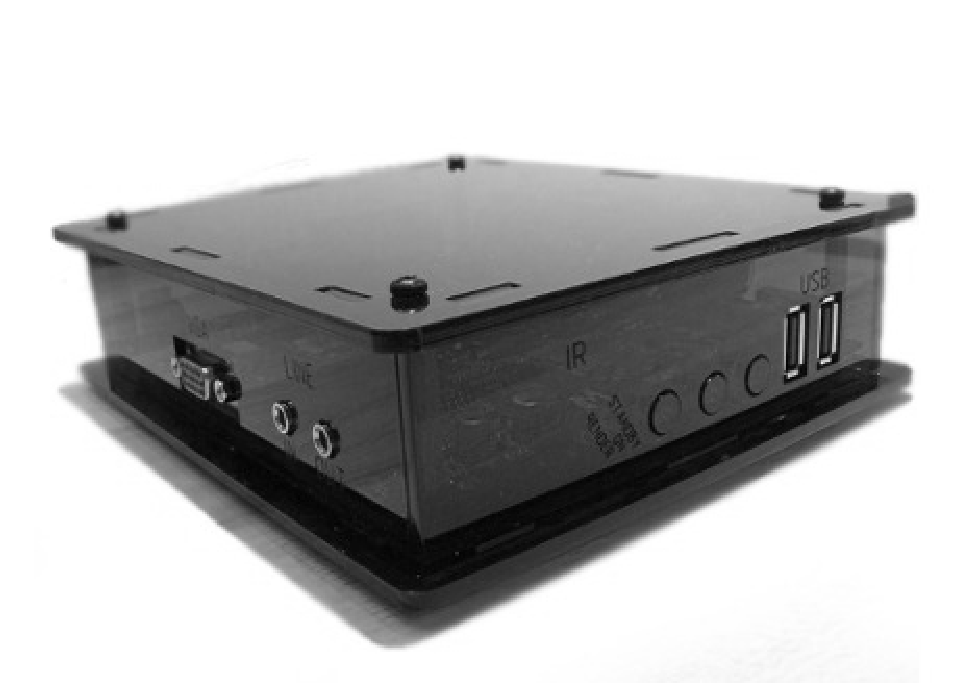
\includegraphics[height=60mm]{mm1_bw.eps}
\caption{Milkymist One (picture: Joachim Steiger, CC-BY-SA)}
\label{fig:mm1}
\end{figure}

\begin{figure}
\centering
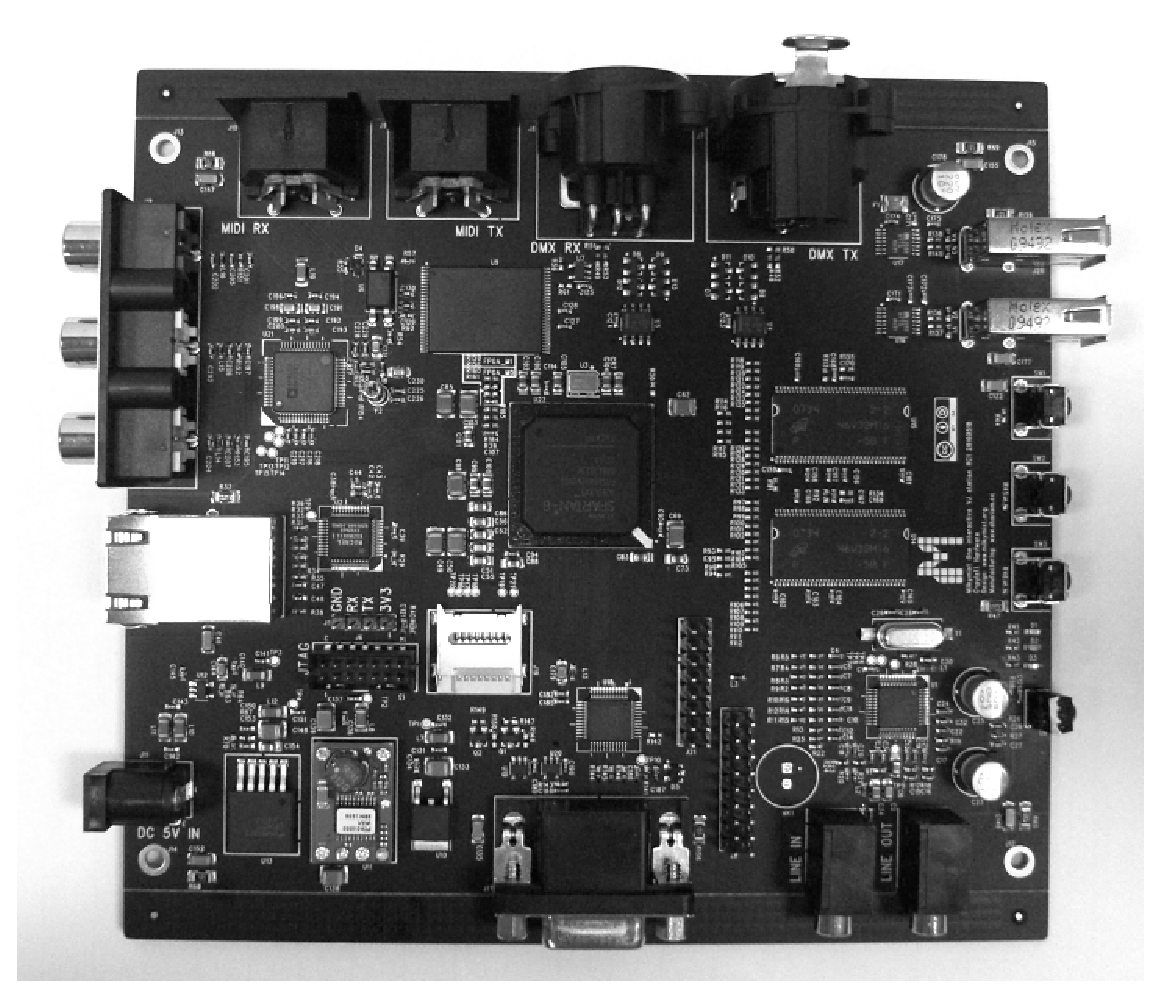
\includegraphics[height=60mm]{mm1nocase_bw.eps}
\caption{Milkymist One, case removed (picture: Adam Wang, CC-BY-SA)}
\label{fig:mm1nocase}
\end{figure}

Early versions of the SoC were prototyped on a Xilinx ML401 development board equipped with a Virtex-4 XC4VLX25 FPGA.

On the software side:
\begin{itemize}
\item ISE Webpack from Xilinx synthesizes the FPGA bitstream,
\item UrJTAG~\cite{urjtag} is used to load bitstreams into the FPGA and write the flash,
\item Verilog simulations are run with GPL Cver~\cite{gplcver} and Icarus Verilog~\cite{icarus},
\item GCC is used to compile the code for the SoC's CPU.
\end{itemize}

All these tools are either free (as in freedom) or available at no charge.

\section{Software support}
As stated earlier, GCC can compile code for the LatticeMico32 CPU target, which eases the porting of existing C or C++ software.

\begin{figure}
\centering
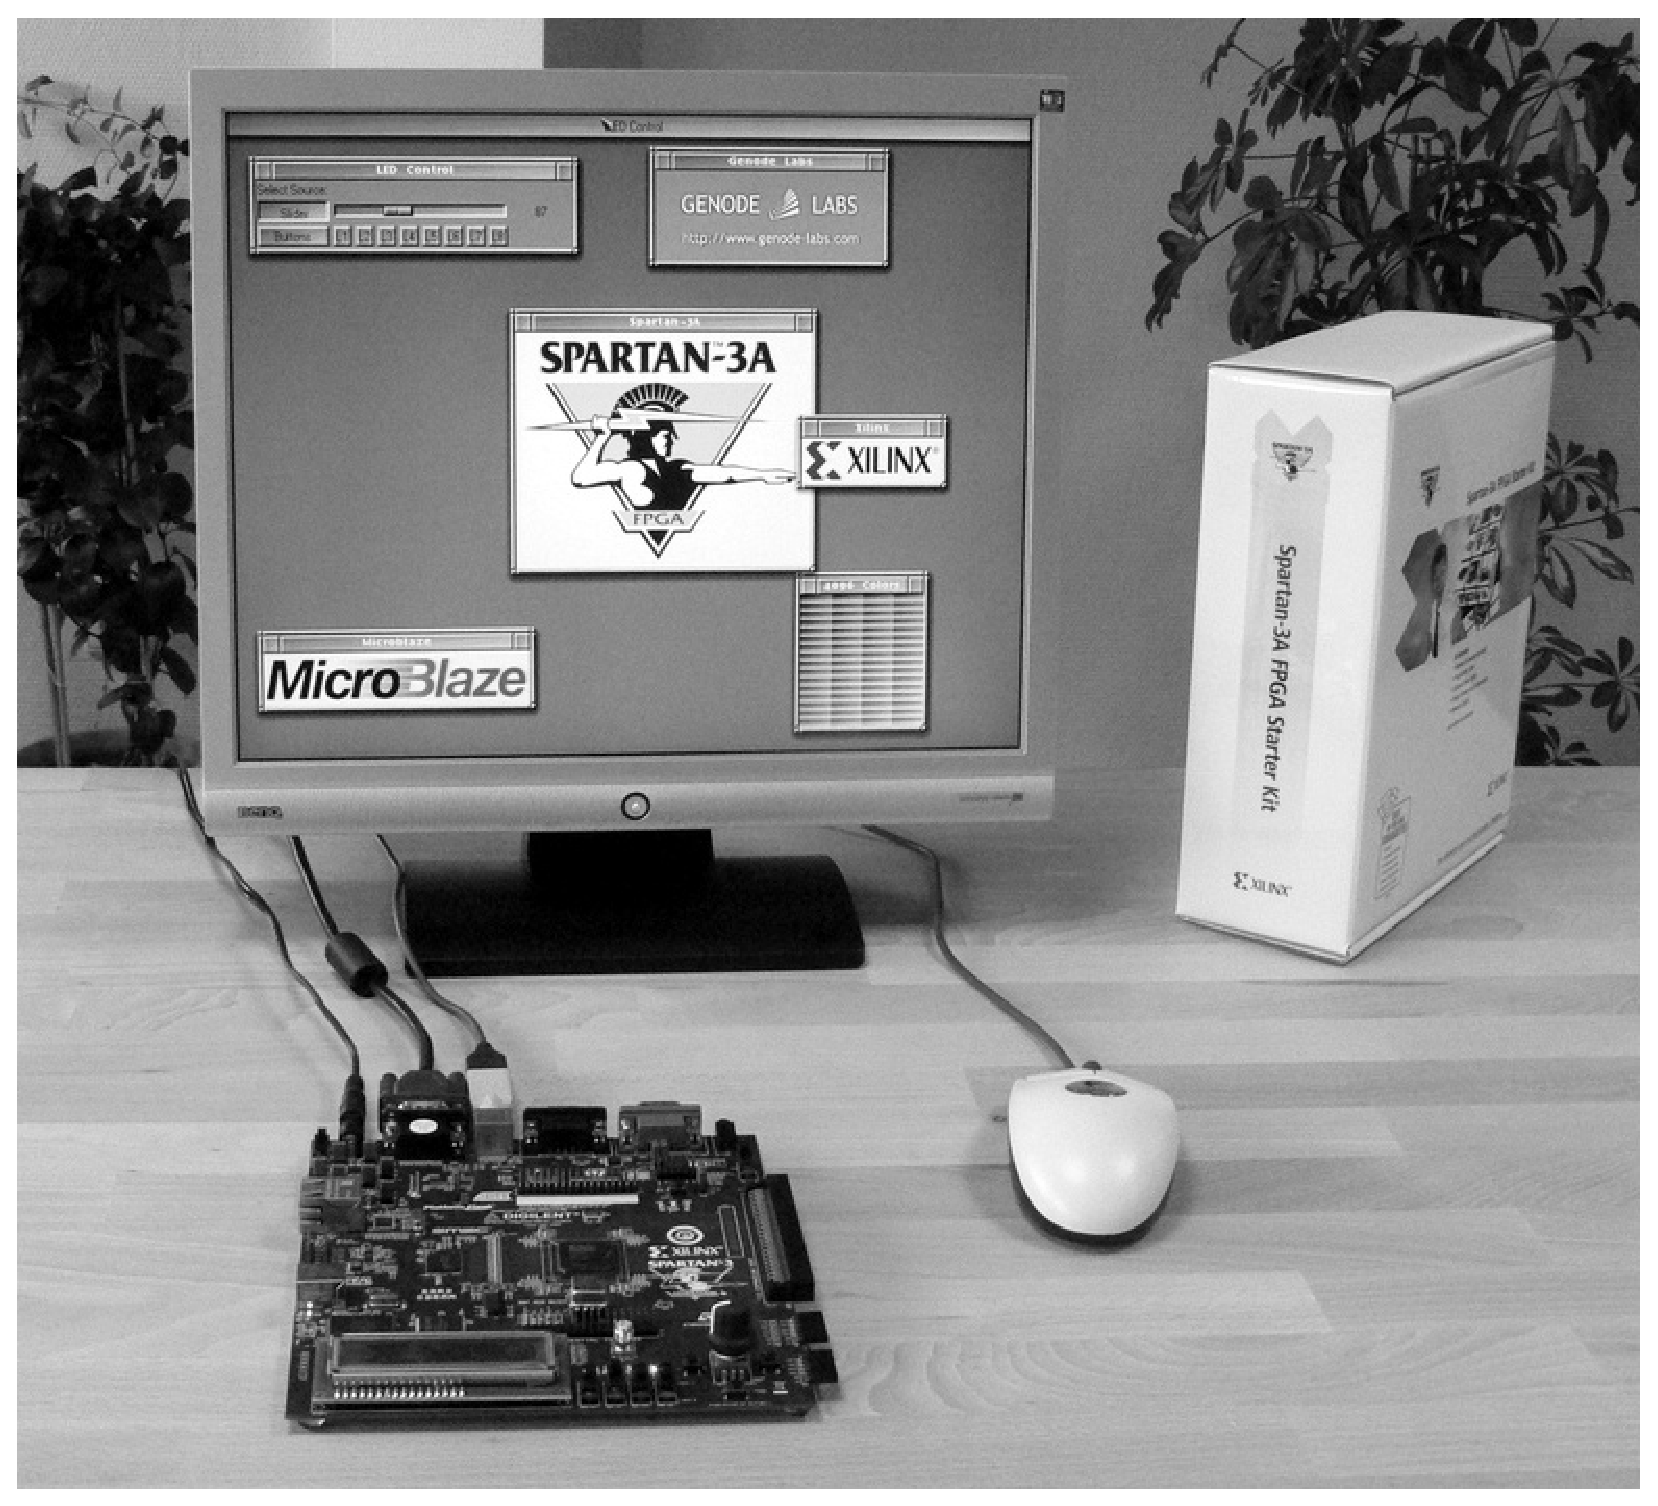
\includegraphics[height=60mm]{genode_bw.eps}
\caption{The Genode FX GUI toolkit (picture: Genode Labs)}
\label{fig:genodefx}
\end{figure}

Our final system runs RTEMS with kernel drivers for all the system-on-chip components, and uses MTK GUI toolkit (which is a modified version the Genode FX GUI toolkit~\cite{genodefx} shown in Figure~\ref{fig:genodefx}) to enable the user to configure and tune the system. The visual effect engine is based on the ``iterative rendering'' idea behind MilkDrop, and uses the same system of parametrizable equations to define the effects.

\section{Conclusion}
Milkymist features a powerful system-on-chip design, perfectly suited for running intensive video processing and graphics applications. It is also fully open-source (GNU GPL license version 3), flexible and well documented, allowing its components to be re-used in other system-on-chip designs.

\section*{Copyright notice}
Copyright \copyright 2007-2011 S\'ebastien Bourdeauducq. Permission is granted to copy, distribute and/or modify this document under the terms of the GNU Free Documentation License, Version 1.3.

\bibliography{paper_overview}{}
\bibliographystyle{plain}

\end{document}
